\documentclass{standalone}
\usepackage{tikz}
\usepackage{amsfonts}
\usepackage{amssymb}
\usepackage{tikzlings}
\usepackage{tikzducks}
\usepackage{hsbcommon}

\begin{document}
    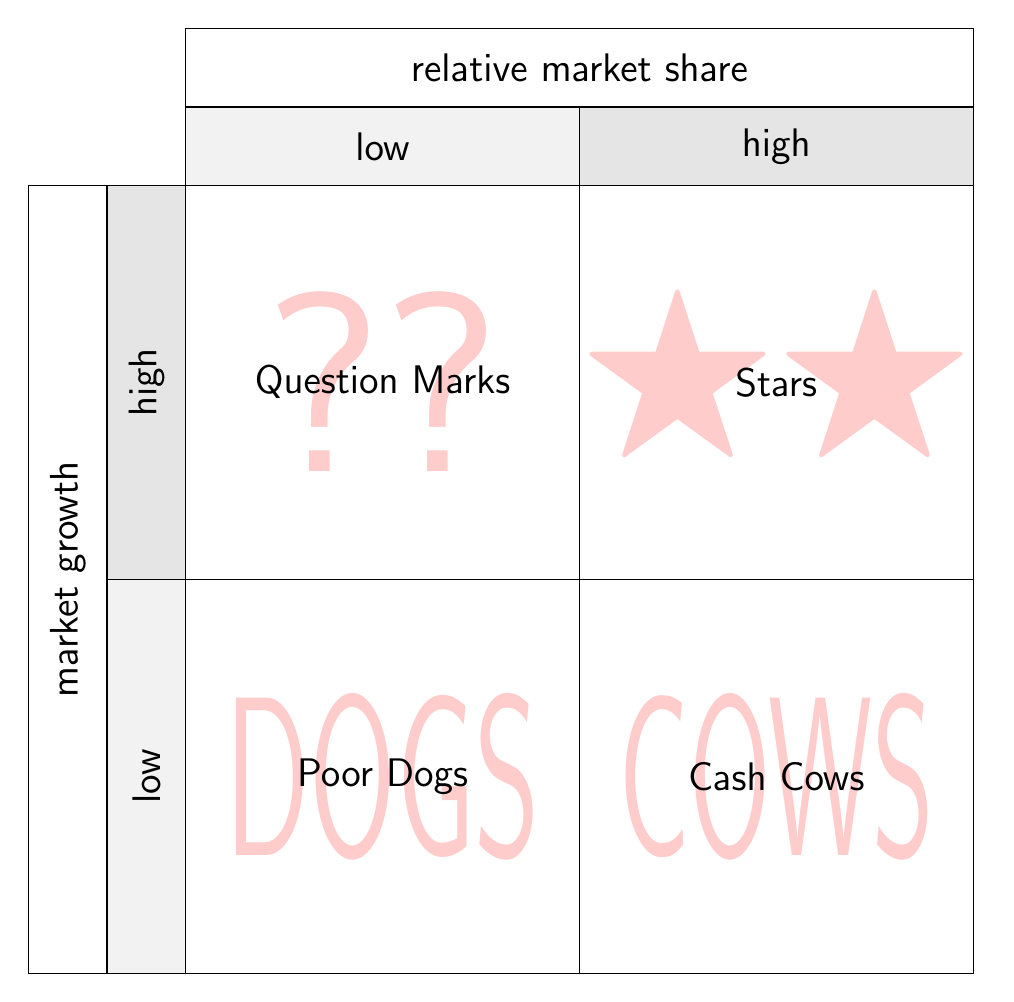
\begin{tikzpicture}[every node/.style={font=\sffamily}]\Large

            \tikzset{every node/.style={
                color=red!20,
                font=\sffamily
            }}
 
            \node (q) at (0,5) {
                \resizebox{3cm}{!}{??}
                };

            \node (s) at (5,5) {
                \resizebox{5cm}{!}{$\bigstar\bigstar$}
                };

            \node (d) at (0,0) {
                \resizebox{4cm}{2cm}{DOGS}
                };

            \node (c) at (5,0) {
                \resizebox{4cm}{2cm}{COWS}
                };

            
            
            \tikzset{
            every node/.style={
                draw,
                text width=15ex,
                minimum height=5cm,
                minimum width=5cm,
                text centered,
                font=\sffamily
            }
        }
        
           \node at (q) {Question Marks};
           \node at (s) {Stars};
           \node at (d) {Poor Dogs};
           \node at (c) {Cash Cows};

            \tikzset{
            every node/.style={
                draw,
                text width=15ex,
                minimum height=1cm,
                minimum width=5cm,
                text centered,
                font=\sffamily
            }
        }

        \node[fill=gray!10] at (q |-,8) {low};
        \node[fill=gray!20] at (s |-,8) {high};
        \node[fill=gray!20,rotate=90] at (-3, |- q) {high};
        \node[fill=gray!10,rotate=90] at (-3, |- d) {low};

            \tikzset{
            every node/.style={
                draw,
                text width=25ex,
                minimum height=1cm,
                minimum width=10cm,
                text centered,
                font=\sffamily
            }
        }


        \node at (2.5,9) {relative market share};
        \node[rotate=90] at (-4,2.5) {market growth};
        
    \end{tikzpicture}
\end{document}